\chapter{Introduction}
\label{chapter:intro}
\graphicspath{{./chapters/c1_intro/figures/}}
%=========== MAIN ================
\begin{abstract}
	Single-molecule fluorescence was invented in the 1990s and has quickly developed into an indispensable technique in the biomedical sciences and condensed-matter research. It has revolutionized the fields of molecular biology, imaging (super-resolution), and catalysis, to name a few. In this thesis, we will apply fluorescence enhancement by single gold nanorods to extend single-molecule studies to chromophores with low fluorescence quantum yields and to high concentrations of probe molecules. Following single-molecule trajectories, we will explore variations in the electron-transfer rates of the metalloprotein azurin both from molecule to molecule and for the same molecule as a function of time. Evidence for conformational substates will be discussed based on dynamic heterogeneity. In this chapter we introduce the basic principles that underlie the research reported in this thesis.
\end{abstract}
\newpage
% =============== MAIN =============
\section{Fluorescence}
The absorption and subsequent emission of light by materials is called fluorescence.
The term fluorescence was named by \textit{George Gabriel Stokes} after he observed the transformation of ultraviolet light into visible light in the mineral fluorite.\cite{Stokes1852} Fluorescence was later observed in organic molecules, and which is the main subject of this work.
A molecule is promoted to an excited electronic state upon absorbing a resonant photon.
Each electronic energy level is associated with vibrational and rotational energy levels.
The excess vibrational energy gained in the excited state is quickly dissipated in the molecular surroundings on picosecond time scales.
The molecule ends up in a thermalized excited state, where it remains for the excited-state lifetime.
Depending on the spin of the excited state, a transition to the singlet ground state may be spin-allowed and lead to fluorescence emission with a lifetime typically of the order of \SIrange{1}{10}{\ns}.
The emitted fluorescent photon has a lower energy than the excitation photon. The associated frequency shift is known as the Stokes shift.
If the excited state is a triplet (spin 1), the transition is spin-forbidden and the lifetime usually lies in the microsecond to seconds range.
The associated emission is called  phosphorescence and is commonly observed at longer wavelengths than the fluorescence.
Absorption and emission processes are often represented graphically in a Jablonski diagram.\cite{RohatgiMukherjee1979k,Lakowicz1999book}

\begin{figure}
	\centering
	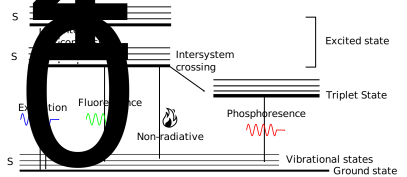
\includegraphics[width=0.8\textwidth]{jablonski}
	\caption{\textbf{Jablonski Diagram.}
	Simplified model of the electronic transitions. A molecule is promoted to the excited electronic state by absorption of a photon.
	Non-radiative relaxation processes bring the molecule to the lowest vibrational state of the lowest excited electronic state from where it can either emit a photon or release excess electronic excitation energy as heat, making a transition to the lower-lying triplet state or singlet ground state.}
	\label{fig:jablonski}
\end{figure}

Natural materials that show fluorescence include minerals and tissues in plants and animals.
Nicotinamide adenine dinucleotide (NADH), flavins (FAD), and chlorophyll are a few examples of common biological molecules that emit significant fluorescence.\cite{blacker2014separating,siano1989nadh,genty1989the}
Alternatively, artificial fluorophores can be synthesized and used for labelling biological structures. These fluorophores present high fluorescence quantum yields and can be produced in a broad variety of colors. They include synthetic organic dyes and semiconductor nanocrystals called quantum dots.\cite{atkinson1952the,alivisatos1996semiconductor}
The greatest advantage of fluorescence is its low background, which enables the detection of exceedingly low concentrations of fluorescent molecules, down to the single-molecule level.
This was important for biological imaging as minute quantities of such markers keep the system under study nearly unaffected.\cite{white1987an}
Not only external fluorophores can be used for biological marking, cells can also be gene-edited to produce their own fluorophores, notably the peptide label called green fluorescent protein (GFP) and a broad variety of similar auto-fluorescent proteins.\cite{tsien1998the,chalfie1994green}
Nowadays, biological or analytical chemical experiments are virtually unthinkable without fluorescence techniques.

\section{Single-molecule spectroscopy}
The thought experiment by Jean Perrin to observe single fluorescent molecules was realized for the first time in 1990 at an extremely low temperature and in an advanced laboratory.\cite{orrit1990single}
The rapid development of optical microscopes, lasers, dyes and detectors soon made it possible to detect single molecules at room temperature even on a bench top.\cite{xie1998optical,weiss1999fluorescence,moerner1999illuminating}
Single-molecule spectroscopy has grown into an important research field, and is heavily used in molecular biology, super-resolution microscopy, quantum computing, and catalysis to name a few fields of application.\cite{zhuang2000a,huang2008threedimensional,eisaman2011invited,lounis2005singlephoton,roeffaers2007singlemolecule}
The following advantages of single-molecule optical microscopy make it an indispensable technique:
\begin{itemize}
	\item \textbf{No averaging.} Ensemble measurements look at the average behavior of vast numbers of molecules, and provide the mean value of a physical quantity.
	In complex media like condensed matter and biological cells, each molecule is in a different microscopic surrounding and experiences different conditions and interactions.
	Single-molecule measurements provide distributions of quantities, revealing sub-populations within the samples under study, presenting distinct characteristics.
	For example, even in a crystalline solid, different guest molecules may exhibit a broad distribution of spectral line shapes and linewidths, indicating the extent of imperfections at molecular scales.\cite{kozankiewicz1994single,reilly1993spectral}
	Differences in the diffusion coefficients of single molecules in a biological membrane possibly indicate small domains of \SIrange{50}{700}{\nm} called membrane rafts.\cite{lommerse2004singlemolecule}
	Rare species that are lost in ensemble measurements can be identified and investigated in single-molecule studies.
	The distribution of parameters observed from molecule to molecule is attributed to static defects in the vicinity of each molecule, an effect called static heterogeneity.
	\item \textbf{Time dependent fluctuations.} Single-molecule methods also enable studies of the dynamics of complex systems without any need for synchronization (kinetic measurements in ensembles require synchronization).
	Single-molecule measurements at equilibrium provide direct access to both dynamics and statistics of molecular complexes.
	They also provide information on a wide range of time scales from microseconds to tens of seconds, displaying translational, orientational, enzymatic-turnovers and protein folding-unfolding events.\cite{schmidt1996imaging,ruiter1997single,lu1998single-molecule,schuler2002probing}
	The distribution of parameters explored along a time trajectory is called dynamic heterogeneity.
	\item \textbf{Local reporter} As single-molecule detection is based on optical microscopy, the observer can be far away from the molecule itself provided the intervening medium is optically transparent. The trajectory of reporter molecules deep inside a cell can be tracked without physical contact, to follow the activity of the host cell.
	\item \textbf{Single molecules as tools} Single molecules are finding applications as tools to perform different tasks. As the transitions in the excitation of single molecules are quantum in nature, they can be used as sources of single photons for quantum communication and computing.\cite{lounis2000single,lounis2005singlephoton}
	Single-step blinking of single molecules is being used for super-localization and imaging down to nanometer-scale resolutions.\cite{park2003superresolution,huang2008threedimensional}
	Moerner, Betzig and Hell were awarded the Nobel Prize in Chemistry in 2014 for their contributions towards super-resolution microscopy and single-molecule detection.
\end{itemize}

Some of the more common applications of single-molecule measurements are discussed above. They can provide a plethora of insights and possibilities are only limited by the practitioner's creativity and imagination.

Two major characteristics that are diagnostic of single molecules are their stepwise changes of intensity and anti-bunching.\cite{rasnik2006nonblinking,basch1992photon}
Molecules in their excited state can cross over to a triplet state, resulting in a loss of emission until the molecule comes back to the ground state, closing the excitation-emission cycle.
This results in blinking, i.e., digital switching of the fluorescence intensity between two levels (see Figure \ref{fig:SM_characteristics}A).
A molecule in its triplet state is more reactive because of its unpaired electrons and can react with triplet oxygen in its surrounding, leading to the formation of singlet oxygen, and thereby to bleaching: the complete loss of fluorescence.
Both one-step blinking and bleaching are used as signature of single molecules.
Single molecules are quantum systems that emit only one photon at a time. When the photon stream from a single molecule is sent to two detectors via a beam splitter, anti-bunching is observed in the cross-correlation of the signals of the two detectors.
Such anti-bunching experiments are known as ``Hanbury-Brown Twiss  measurements'' and are currently used to demonstrate that a source emits photons one by one, as a single emitter.\cite{brown1956correlation}
\begin{figure}
	\centering
	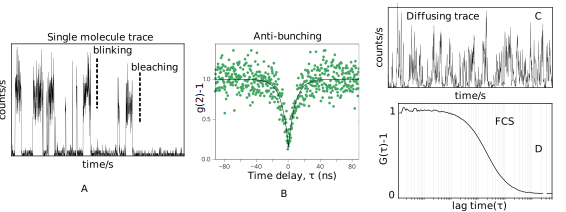
\includegraphics[width=\textwidth]{SM_characteristics}
	\caption{\textbf{Single-molecule characteristics.}
	(A) Time trace of a single molecule showing single-step switching (blinking) and bleaching.
	Notice the reappearance of the intensity after blinking but its irreversible disappearance upon bleaching.
	(B) Anti-bunching at zero delay time in the correlation shows that the photons are emitted by a single emitter.\cite{chu2016a}
	(C) Time trace of diffusing molecules in a fluid with \SI{1}{\nM} fluorophores, showing intensity bursts and the large correlation amplitude ($G(\tau)-1={\sim}1$) indicating the presence of a few molecules in the focus.}
	\label{fig:SM_characteristics}
\end{figure}

Fluorescence correlation spectroscopy (FCS) is often considered as a single-molecule technique. It measures the temporal correlation of fluctuating light intensities.\cite{magde1972thermodynamic,elson1974fluorescence,krichevsky2002fluorescence}
The conventional way to perform FCS is to collect the signal from \textit{diffusing fluorescent} molecules in the diffraction-limited focal volume and then to compute the autocorrelation of the intensity trajectory.
The autocorrelation of the intensity signal is given as $G(\tau)=<I(t)I(t+\tau)>/<I(t)>^2$ where I is the intensity, $\tau$ the lag time and $<...>$ represents time averaging.
The correlation quantifies the probability that the intensity at time $t$ is similar to the intensity at a later time $t+\tau$.
It provides information on the concentration and the time scale of the fluctuating observable.
By its very nature, FCS requires fluctuation of the number of diffusing fluorophores in the diffraction-limited volume of \SI{1}{fL}, preferably a number in the order of one molecule per focal volume on average.
Because of the diffraction limit ($\Delta{x}={\lambda}/2$), FCS is often limited to nanomolar and picomolar concentrations of the analyte.

Two of the important requirements to measure single molecules with high spatial and temporal resolution are (i) high fluorescence yield and (ii) small excitation and detection volumes.
In this thesis we push the limit of single-molecule detection to low quantum yield dyes and to high concentrations of fluorophores.

\section{Time-correlated single-photon counting (TCSPC)}
Fluorescence signals are normally recorded as fluorescence intensity and are obtained by recording a photodiode voltage as a function of time.
The advancement in sensitive detectors enabled the detection of individual quanta of light, with single-photon counting units.
Detailed information about a single molecule can be extracted when all the photon detection events are registered in time.
The time-resolved technique used to record the information about photons is known as Time-Correlated Single-Photon Counting (TCSPC).\cite{oconnor2012timecorrelated,birch2002topics}
This technique requires a pulsed laser with high repetition rate (\SI{\sim80}{\MHz}) and a short pulse duration (picoseconds).
TCSPC is suitable for small signals with less than one photon on average per laser pulse.
With each laser pulse, there is a probability of excitation of the molecule, which depends on the excitation cross section, and the intensity of the laser.
Once excited, the molecule may emit a photon with a probability depending on the radiative ($\Gamma_{r}$) and nonradiative ($\Gamma_{nr}$) rates of excited state relaxation.
The fluorescence lifetime can be given as:
\begin{equation}
	\tau_f = \frac{1}{\Gamma_{r} + \Gamma_{nr}}
\end{equation}
The arrival time of the emitted photon after the exciting laser pulse is called microtime (t\_micro) and the absolute arrival time from the start of the measurement is called macrotime (t\_macro).
\begin{figure}
	\centering
	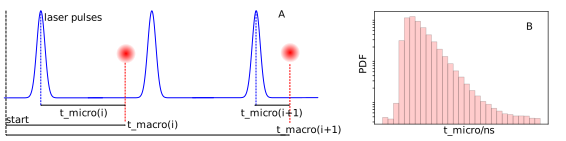
\includegraphics[width=\textwidth]{tcspc_sch}
	\caption{\textbf{TCSPC.} (A) The scheme of a time-resolved experiment showing the laser intensity trace (blue curve) and the subsequently detected photons as the red dots.
	The arrival time of emitted photons after the laser pulse is called microtime and the arrival date after the start of measurement is called macrotime.
	(B) The histogram of the micro-times gives the life time of the fluorophores.}
	\label{fig:tcspc_sch}
\end{figure}
The advantages of TCSPC measurements can be summarized as follows:
\begin{itemize}
	\item \textbf{Binning-free data.} As each photon is recorded with its arrival time, TCSPC is binning-free, unlike the intensity measurements.
	From the photon arrival time, intensity traces with any binning time can be produced after the measurement.
	The accessible dynamic range is limited at short times (picoseconds) by the resolution of the detector and the laser pulse duration, and for long times by the total recording time.
	Fluorescence correlation spectroscopy (FCS) utilizes the information provided by TCSPC and displays dynamics occurring over many orders of time in a single autocorrelation curve, often plotted on a logarithmic time scale.
	\item \textbf{Lifetime.} The distribution of photon delays after excitation (t\_micro) often follows a single-exponential distribution with an average fluorescence lifetime, which can be obtained by fitting the histogram of microtimes (Figure \ref{fig:tcspc_sch}B).
	The lifetime can not only give the intrinsic decay rate of the excited fluorophore, it also carries information about the immediate surroundings with which the dye interacts.
	Other applications of lifetime measurements are fluorescence resonance energy transfer (FRET) and fluorescence lifetime imaging.\cite{selvin2000the,lakowicz1992fluorescence} 
	\item \textbf{Linking of microtime and macrotime.} As each photon is stamped with microtime and macrotime, correlations can be extracted between the lifetime and dynamics of the macromolecules.
	Multiple fluorophores in a system can be distinguished on the basis of their fluorescence lifetimes.
\end{itemize}
In this thesis, almost every fluorescence measurement was done with both microtime and macrotime information.
In Chapter 2, both micro and macro times are used to distinguish the shorter lifetime photons from the longer lifetime photons to enhance the visibility of correlation in FCS experiments.
Chapter 3 utilizes the inter-photon times (t\_macro(i+1) - t\_macro(i)) to extract information that can be misrepresented by the binning methods.
In chapter 4, the potential of TCSPC is tested to explore dynamical heterogeneity in an electron-transfer protein. 


\section{Optical nano-antennas for single molecules}
Single-molecule fluorescence spectroscopy is usually limited to fluorophores with high quantum yield (\SI{>10}{\percent}) and to low concentrations of molecules (\SI{}{\pM-nM}).
A large fraction of absorbing molecules including biomolecules and metal complexes show weak fluorescence with very low quantum yield (\SI{<1}{\percent}).
Background auto-fluorescence in physiological conditions often reduces the signal-to-noise ratio.
In addition, a majority of physiological reactions involving proteins and enzymes require milli- to micro-molar concentrations of substrates and cofactors.\cite{craighead2006future,punj2013gold,fabrizio2016roadmap,punj2014thesis}
Thus, systems at physiological conditions with micromolar concentrations cannot be studied conveniently by conventional single-molecule fluorescence microscopy.
Nano-plasmonics offer a promising solution to these problems by lifting the concentration limit by light confinement in the optical near field, and by enhancing the emission rate of dyes with poor fluorescence quantum yields.


Optical nano-antennas are similar to radio antennas at the macro scale.
Antennas are used to control and manipulate electromagnetic (EM) waves on the sub-wavelength scale.
Currents from a transmitter can be coupled to an antenna and radiated as EM wave to the far-field while on the other end EM waves in the far-field can be coupled to the antenna and sent to the receiver (Figure \ref{fig:nano_antenna}A,B).
Marconi used antennas with sizes of about ten meters to control waves with kilometer wavelength. 
Similarly, nanoscale antennas can be used to control optical waves with sub-micrometer wavelengths.
Nano-antennas present resonant modes called surface plasmon resonances (SPR's), involving collective motion of the metal's free electrons.
Excitation of these surface plasmon resonances provide strong near-field enhancements, confining electromagnetic waves to local hot spots. \cite{bath8624,schuller2010plasmonics,ozbay2006plasmonics,maier2005plasmonics,hess2012active}
In addition to the SPR effect, the local electric field is also enhanced by the lightning rod effect, which is a result of the high charge density at the edges or sharply curved tips of the antennas.
Compared to the diffraction limit of light, of order $\lambda/2$, plasmonics can confine light down to much smaller spots, even less than nanometers in geometries with nanoparticles on a mirror\cite{benz2016singlemolecule}.
\begin{figure}
	\centering
	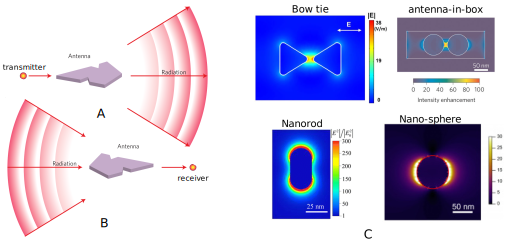
\includegraphics[width=\textwidth]{nano_antenna}
	\caption{\textbf{Optical nano-antenna.} Antenna coupled to the emitter or transmitter (A) and receiver (B). The direction of energy flow is shown by the arrows.
	Antennas help convert free propagating light waves to localized energy and help radiate localized energy into the far-field.
	(C) Examples of nano antennas with their enhanced electric field.
	The color scales are an indication of the electric field ($|E|$) or its intensity ($|E|^2$), as indicated close to each nano-structure. (A) and (B) was reprinted from ref \cite{novotny2011antennas}. (C) was reprinted from \cite{kinkhabwala2009large,punj2013a,khatua2014resonant}}
	\label{fig:nano_antenna}
\end{figure}

The fluorescence of an emitter placed in the near-field of a nano-antenna will be enhanced (i) by enhanced excitation in the high near field and (ii) by enhancement of the radiative decay rate.
Because of the high light intensity in the near-field, the fluorophore will be pumped harder. This effect is known as excitation enhancement.
The transition probability of an emitter governed by Fermi's Golden rule depends on the local density of states (LDOS) in addition to the transition matrix element between the two states.
Nano-antennas significantly modify the LDOS enhancing the radiative rates of the emitter, leading increased spontaneous emission. This effect is known as radiative enhancement.
Close to the metal surface, additional non-radiative channels lead to quenching of fluorescence via Ohmic losses.
Thus the resultant enhancement depends upon the emitter's position and orientation with respect to the antenna, and on the overlap of its emission spectrum with the resonance of the antenna.\cite{anger2006enhancement,khatua2014resonant}

The strength of the field enhancement and the field spatial distribution depend on the nanostructure, as shown in the examples of Figure \ref{fig:nano_antenna}C.
The quality of an antenna is judged by the large field enhancement factor and smaller mode volume.
Bow tie antennas and antennas-in-box provide high field enhancements and small near-field volumes but require tedious and expensive lithographic expertise.\cite{novotny2011antennas,regmi2017thesis}

A gold nano-sphere is the most straightforward example of a nano-antenna, but it gives low field enhancement and large near-field volume.\cite{punj2013gold}
Gold nanorods are somewhat better antennas because of their larger field enhancement and have a somewhat larger field confinement compared to nanospheres.
Moreover, they present a stronger and narrower spectral response than spheres. For the research described in this thesis, gold nanorods are our favorite nano-antennas because:
\begin{itemize}
	\item Their field enhancement is comparable to that of the best antennas available.
	\item The plasmon resonance can be tuned from green to far-infrared simply by changing the aspect ratio of the rod.\cite{link1999simulation}
	The spectral width of the plasmon is relatively small and the light-confinement volume can be controlled to some extent by changing the volume of the rod.
	The narrow surface plasmon resonance is helpful for selective enhancement of emitters.\cite{yuan2013thousandfold,khatua2014resonant}
	\item Gold nanorods can be cheaply mass-produced by colloidal synthesis with high crystalline quality and smooth surfaces.\cite{nikoobakht2003preparation,perezjuste2005gold}
	\item Accessibility. As nanorods are small and colloidal in nature, they can be easily inserted into living cells.\cite{el2005surface,chithrani2007elucidating,pan2007size,lvy2010gold,moser2016cellular}
	In fact, because of their photoluminescence, they are being used in living cells or tissues for imaging.
	\item Selective reactivity. Gold is inert and harmless for living organisms unlike other metals like silver.
	It has high affinity towards thiols, opening the possibility of chemical functionalization.
\end{itemize}
%
\section{Proteins at work are proteins in motion}

Proteins and enzymes are the machines inside living cells that perform vital functions, including mechanical work and energy maintenance.
Proteins and enzymes are often pictured by their static structures obtained by crystallography or the average structure of a large ensemble of conformations obtained from NMR spectroscopy.
The functions of a protein are governed by its dynamical motions.
A multidimensional energy landscape and different kinetic barriers govern the complex coordinated motion of proteins.
To understand how protein function is related to structure and dynamics, we need to follow their physical properties in the fourth dimension, time.
Enzymes perform chemical reactions by binding with their substrate and minimizing the energy barrier, which needs to be overcome for product formation.
Spectroscopic studies done in the 1980's and recent nuclear magnetic resonance (NMR) investigations show the amplitude and duration of structural fluctuations involved in the function of enzyme catalysis and protein function.
Movements are observed on time scales ranging from picoseconds corresponding to atomic movements to milliseconds involving movement of bigger domains.\cite{henzler-wildman2007dynamic,frauenfelder1991the}
The time scale of transitions relates to the energy barriers between different conformations. Those are represented as a free-energy landscape of a multidimensional space of reaction coordinates.
The concept of energy landscape was first introduced by Frauenfelder and co-workers\cite{frauenfelder1991the} to explain the observation of multiple energy barriers and non-exponential kinetics in the rebinding of carbon monoxide and oxygen to myoglobin.
They connected the myoglobin function to the energy barriers and the existence of conformational sub-states.
Since then, other studies by NMR and single-molecule techniques have advanced our knowledge about the protein energy landscapes.

\begin{SCfigure}[0.9][ht] %this figure will be at the right
    \centering
    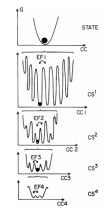
\includegraphics[width=0.4\textwidth]{energy_landscape}
    \caption{\textbf{Hierarchical arrangement of the conformational substates.} The energy landscape of a protein shows hierarchical protein dynamics and energy barriers. The upper diagram shows an energy minimum representing a state of the protein. Zooming in on that state, we find more substates, which themselves subdivide into more and more conformational substates at higher and higher order of energy. Up to four tiers have been defined in the hierarchy of conformational substates. The figure was reprinted from ref \cite{ansari1985protein}}
    \label{fig:energy_landscape}
\end{SCfigure}

An energy landscape is defined as a map of all possible atomic positions in a molecule and their corresponding Gibbs free energy.
The very complex multidimensional energy landscape is typically represented in a two-dimensional conformational coordinate (cc) system.
The hypersurface of energy landscape consists of a number of valleys. Each free-energy minimum corresponding to the initial and final state of a reaction is called a ``state'', while each saddle point between two minima is known as a ``transition state''.
Each state can assume a very large number of conformational substates, which can be hierarchically ordered into different tiers of energy (Figure \ref{fig:energy_landscape}).
The transition time directly relates to the energy barriers, the transitions in the tier-4 ($CS^4$) occur in a shorter time than in the tier-0($CS^0$).
Protein motions can be categorized mainly into two types- equilibrium fluctuations (EF) and  functionally important motions (FIMs).\cite{ansari1985protein}
EFs involve motions among the substates and result in equilibrium thermodynamic properties like entropy and internal energy. 
Examples of equilibrium fluctuations include bond vibration, methyl rotation, loop motion and side-chain conformational changes.
Larger changes in the structure during functionally important movements may bring the protein to different substates.
Any reaction whose rate depends on the conformational substate will thus exhibit rate fluctuations, leading to non-exponential kinetics and dynamical heterogeneity.
In this thesis, we will investigate the rate of complex formation between an electron transfer protein and redox chemicals in solution.
We will attribute variation in the rates, i.e., the dynamical heterogeneity, to conformational changes.

\section{Azurin: an electron-transfer protein}
Electron transfer via oxidation and reduction controls vital cellular processes like respiration, redox homeostasis, and photosynthesis, to name a few.
Proteins with a metal co-factor play a crucial role in carrying out such electron transfers.
Among the metalloproteins, copper and iron containing proteins are most common.
They carry out activities like oxygen transport (hemocyanin), respiration (cytochrom-c oxidase) and metal homeostasis (ceruloplasmin).
Because of their electron-transport properties, metalloproteins are promising candidate for biosensors and biomolecular electronic devices.


Azurin is a copper-containing protein involved in electron transfer in cells.\cite{dennison2005investigating,kolczak2006handbook}
The copper ion is buried in the so-called northern part of azurin (MW=\SI{14}{\kilo\dalton}).
It is surrounded by a coordination sphere composed of two histidines, a cysteine and methionine (Figure \ref{fig:azurin_structure}(B)).
The copper atom in azurin can be in either of two oxidation states: Cu(II) and Cu(I).
Cu(II) azurin has a blue color due to an absorption at \SIrange{595}{630}{\nm} arising from a $\pi - \pi^*$ transition in the molecular orbital scheme of azurin.\cite{dooley1981spectroscopic,schmauder2005sensitive}
In contrast, Cu(I) azurin is colorless as it has no absorption band in the red(Figure \ref{fig:flurox_azurin}).
The different spectroscopic characteristics of the two states of Cu can be used to measure the kinetics of electron transfer of azurin.
The oxidation and reduction reactions via electron transfer are generally known as redox reactions.
The redox properties of azurin are determined by the Cu atom and the ligands surrounding Cu.
Azurin has a midpoint potential of \SI{60}{\mV}(vs the Saturated Calomel Electrode, SCE) at pH 7.
Azurin is well characterized and is a reasonably stable protein at room temperature, which makes it a suitable candidate for investigating fundamental properties of electron-transfer reactions.
\begin{figure}
	\centering
	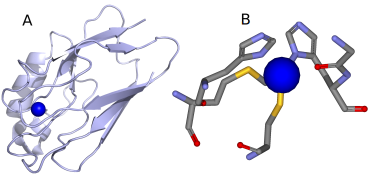
\includegraphics[width=\textwidth]{azurin_structure}
	\caption{\textbf{Azurin structure.} (A) Crystal structure (cartoon representation) of azurin from \textit{Pseudomonas aeruginosa}.\cite{adman1981structural}
	The copper atom is shown as a blue sphere.
	(B) Ligands around copper atom: His117, His46, Cys112, Met121}
	\label{fig:azurin_structure}
\end{figure}


\section{FluRedox principle (FRET-redox)}
The absorption band at \SIrange{595}{630}{\nm} of azurin has been used to study electron-transfer kinetics in ensembles.
To study electron transfer in single azurin molecules, a more sensitive background-free fluorescence-technique in the red-infrared range can be used.
Azurin does not have intrinsic fluorescence in the red spectral range.
When the external fluorescent marker ATTO655 is attached, the emission spectrum matches (see Figure~\ref{fig:flurox_azurin}) with the absorption of Cu(II) azurin, the dye fluorescence will be quenched when the protein is in the oxidized state, whereas the fluorescence in Cu(I) form will be bright due to the absence of quenching.
In other words, the oxidation state of the azurin can be read out simply by looking at the fluorescence of labeled azurin.
The principle to detect the oxidation state in metalloenzymes by looking at the fluorescence of an external marker is called FluRedox. It was pioneered by Aartsma, Canters and co-workers.\cite{kuznetsova2008the,goldsmith2011redox,tabares2011fluorescence}
\begin{figure}
	\centering
	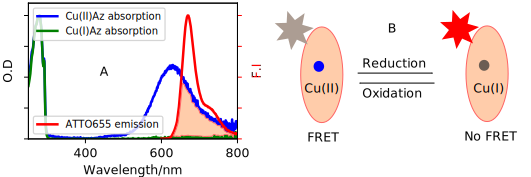
\includegraphics[width=\textwidth]{flurox_azurin}
	\caption{\textbf{Fluorox principle.} (A) Spectral overlap between the absorption of azurin and the emission of ATTO655. Blue curve: absorption of Cu(II) azurin, green: absorption of Cu(I) azurin, red: emission of ATTO655.
	(B) Symbolic representation of the fluorescent state of azurin-ATTO655 in Cu(II)-state and Cu(I) state. In the Cu(II) state, copper is shown as a blue sphere and the non-fluorescent ATTO655 is shown in light gray. In the Cu(I) state, copper is shown in green and the fluorescent ATTO655 is shown in red.}
	\label{fig:flurox_azurin}
\end{figure}
The efficiency of fluorescence quenching can be calculated as in fluorescence resonance energy transfer (FRET). It is given by:
\begin{equation}
	E = \frac{R_0^6}{R_0^6 + r^6}	
\end{equation}
where $r$ is the distance between the Cu-atom and the dye, and $R_0$, called the $F\ddot{o}rster$ radius, is the distance at which the efficiency is \SI{50}{\percent}.
The $F\ddot{o}rster$ radius can be given as:
\begin{equation}
	R_0 = 0.211[\kappa^2n^{-4}Q_DJ(\lambda)]^{1/6}	
\end{equation}
where $\kappa^2$ is an orientation factor, $n$ the refractive index of the solvent, $Q_D$ the quantum yield of the label and $J(\lambda)$ the spectral overlap between the absorption of azurin and the emission of the dye.
The overlap between the emission of the dye ATTO655 and the absorption of azurin can be visually seen in Figure~\ref{fig:flurox_azurin}A.
When ATTO655 is attached at the Lys122 of azurin, the quenching efficiency is around \SI{90}{\percent}.
Such high quenching efficiency allows us to study electron transfer and its heterogeneity at the single-molecule level(Chapter~5).

\section{This thesis}
The common theme of this work is single-molecule fluorescence. In the first part of the thesis, we try to improve signals from single molecules by plasmonic fluorescence enhancement, and to characterize the near field of the plasmonic structures from the statistics of enhanced signals. In the second part, we use the potential of single-molecule microscopy to gain insight into changes of conformational substates, by looking at the electron-transfer dynamics in azurin.

\begin{itemize}
	\item \textbf{Chapter 2.} Many physiological reactions like enzyme-substrate reactions occur in millimolar to micromolar concentrations.
	Single-molecule studies do not provide direct access to such high concentrations because there are still thousands of molecules in the diffraction-limited detection volume of a few femtoliters.
	In this chapter, we use gold nanorods to perform fluorescence correlation spectroscopy at physiologically relevant concentrations.
	The gold nanorod helps to confine light to smaller volumes and enhances the dye fluorescence.
	The fluorescent probe molecules (ATTO647N) were allowed to freely diffuse in a supported lipid bilayer.
	The zwitterionic head groups on the lipid prevent any non-specific interaction between the substrate and the gold nanorod.
	Similar diffusion coefficients were observed in the far-field and near-field suggesting the absence of influence of the gold nanorod on the dye diffusion.
	The diffusion times in the near-field and far-field allowed us to determine the extent of the near field of the gold nanorod.
	The fluorescence of the dye was enhanced by a maximum factor of five.
	The lower enhancement factor was attributed to the inaccessibility of the diffusing dyes to the hottest spot in the near field and to the high quantum yield of the probe (\SI{70}{\percent}).
	The enhanced dyes had a shorter lifetime than the un-enhanced dyes.
	By filtering out fluorescence signal with longer lifetime, the correlation contrast was improved by more than two orders of magnitude.
	We also functionalized the bilayer with azurin-ATTO655 (biomolecule) and obtained a similar improvement in the correlation contrast without any nonspecific interaction with the substrate.
	
	\item \textbf{Chapter 3.} The fluorescence enhancement factor by a single plasmonic structure varies strongly  (up to three orders of magnitude) depending on the position and orientation of the fluorescent probe.
	Furthermore, fluorescence bleaching limits the number of single molecules to one per single nanorod (in a single-molecule study).
	In this chapter we use transient binding by DNA to repeatedly and reproducibly study many single molecules on a single nanorod on the same spot on its tip.
	The longer persistence length of DNA helps to keep the dye at a fixed distance from the tip. We optimized the passivation of the gold nanorod surface to control the average number of binding sites down to one and to minimize fluctuations of the intensity of the enhanced fluorescence.

	\item \textbf{Chapter 4.} A more general way to characterize single-molecule time traces is to bin the trace and look for histograms of intensities and durations of the transitions.
	The enhancement factor extracted from the time traces in the presence of a gold nanorod were different for different binning times.
	We investigated the interphoton times to extract an average enhancement factor and the number of molecules in the near field.
	We performed numerical simulations and employed theoretical models to extract the intensity distribution for slowly diffusing molecules in a two-dimensional bilayer.
	The non-exponential character of the interphoton-time distribution was found to strongly depend on the average number of molecules in the near field.
	Enhancement factors were estimated for diffusing dyes around a gold nanorod and compared with the enhancement factors obtained from binning.

	\item \textbf{Chapter 5.} In the final chapter, we investigated electron transfer in redox active single azurins.
	The oxidation state of the Cu-azurin was read out by observing the brightness of the fluorophore.
	Switching of copper oxidation state was studied at different redox potentials where the potential was controlled electrochemically by a potentiostat.
	The distribution of midpoint potentials was characterized both spatially and dynamically (longer time traces).
	The rate of complex formation between azurin and its redox partners showed correlated variations in time.
	As the variations were observed in steady state conditions and on a passive functionalized glass surface, the heterogeneity was attributed to the different conformations (substates) of azurin.
\end{itemize}
% \references{bibliography}=